\documentclass{article}

\usepackage[margin=1.0in]{geometry}
\usepackage{marginnote}
\usepackage{listings}
\usepackage{tikz-qtree}
\usepackage{tikz}
\usepackage{wrapfig}
\usepackage{caption}
\usetikzlibrary{shapes, arrows, positioning, calc, matrix, chains, trees, positioning,automata}

%\newcommand{\thickbox}[1]{\fbox{{\bf #1}}}
\newcommand{\thickbox}[1]{\setlength{\fboxrule}{1.3pt}\fbox{#1}\setlength{\fboxrule}{0.4pt}}

\lstdefinelanguage{Pseudo}
{keywords={if, return, function,length, for, each, else, join, in, swap, or ,and}}

\lstdefinestyle{pseudo}{
	language=Pseudo,
	aboveskip=3mm,
	belowskip=3mm,
	columns=flexible,
	basicstyle={\normalsize\ttfamily},
	keywordstyle=\bf,
	numbers=none,
	frame=none,
	breaklines=true,
	breakatwhitespace=true,
	stepnumber=2,
	tabsize=4
}


\begin{document}
\reversemarginpar

\title{Computer Science Compendium}
\author{Scott Tolksdorf}
\maketitle
\clearpage
\setcounter{tocdepth}{2}
\tableofcontents
\clearpage
\section{Introduction}

\clearpage
\section{Sorting}

%-----------------------------------------------------------------------------------------------------------------

\subsection{MergeSort}
\marginnote{\scriptsize{CLRS pg.31}}
MergeSort is a {\bf Divide and Conquer algorithm}, it's recursive and can be parallelized well between multiple processors. It has {\bf Stable Sorting}, so items with the same value perserve their order from the original list. {\bf Best/Worst Case} $O(n \log n)$ and {\bf Aux. Space} of  $\Omega(n)$. {\bf Best used} when accessing data sequentially is important, eg. parallel/external sorting. On average slower then HeapSort and QuickSort.
\\ \\
MergeSort splits its list until it's down to 1 element, then rejoins them recursively inorder.

\begin{wrapfigure}{r}{2cm}
	\begin{tikzpicture}
	[scale=1.0, transform canvas={scale=1.0},
	node distance=0.2cm and 0.07cm,
	every node/.style={align=center}]
	\node (s0) {\fbox{6}\fbox{2}\fbox{1}\fbox{5}};
	\node[below left=of s0] (s1a) {\fbox{6}\fbox{2}};
	\node[below right=of s0] (s1b) {\fbox{1}\fbox{5}};
	\node[below left=of s1a] (s2a) {\fbox{6}};
	\node[below right=of s1a] (s2b) {\fbox{2}};
	\node[below left=of s1b] (s2c) {\fbox{1}};
	\node[below right=of s1b] (s2d) {\fbox{5}};
	\node[below right=of s2a] (s3a) {\fbox{2}\fbox{6}};
	\node[below left=of s2d] (s3b) {\fbox{1}\fbox{5}};
	\node[below left=of s3b] (s4) {\fbox{1}\fbox{2}\fbox{5}\fbox{6}};
	\foreach \from/\to in {
		s0/s1a,s0/s1b,
		s1a/s2a,s1a/s2b,s1b/s2c,s1b/s2d,
		s2a/s3a,s2b/s3a,s2c/s3b,s2d/s3b,
		s3a/s4,s3b/s4}
		\draw[->] (\from) -- (\to);
	\end{tikzpicture}
\end{wrapfigure}
\begin{lstlisting}[style=pseudo]
function MergeSort(list)
	if length(list) <= 1
		return list
	split list -> A, B
	A = MergeSort(A), B = MergeSort(B)
	loop through each A, B and merge in sorted order
	return result
\end{lstlisting}

\vspace{10 mm}

%-----------------------------------------------------------------------------------------------------------------

\subsection{QuickSort}
\marginnote{\scriptsize{CLRS pg.170}}
QuickSort is a {\bf Divide and Conquer algorithm}, it's recursive and can be parallelized well between multiple processors. It has {\bf Non-Stable Sorting}, so items with the same value do not perserve their order from the original list. {\bf Best Case} $O(n \log n)$, {\bf Worst Case} $O(n^2)$ and {\bf Aux. Space} $\Omega(\log n)$. {\bf Best used} when speed is top priority. Can have cases where running time is very slow, bad for very large data sets and possible for attacks.
\\ \\
QuickSort chooses a pivot, then creates two new lists, one containing elements less then the pivot and one greater then the pivot. Recursively applies this to the new lists. Rejoins them with the pivot.


\begin{wrapfigure}{r}{2cm}
\begin{tikzpicture}
[scale=1.0,
transform canvas={scale=1.0},
node distance=0.2cm and 0.04cm,
every node/.style={align=center}]
\node (s0) {\fbox{5}\fbox{2}\thickbox{3}\fbox{1}\fbox{6}};
\node[below left=of  s0] (s1a) {\thickbox{2}\fbox{1}};
\node[below right=of s0] (s1c) {\thickbox{5}\fbox{6}};

\node[below left=of  s1a] (s2a) {\fbox{1}};
\node[below =of      s1a] (s2b) {\thickbox{2}};
\node[below right=of s1a] (s2c) {\fbox{\phantom{0}}};

\node[below left=of  s1c] (s2d) {\fbox{\phantom{0}}};
\node[below =of      s1c] (s2e) {\thickbox{5}};
\node[below right=of s1c] (s2f) {\fbox{6}};

\node[below =of s2c] (s3a) {\fbox{1}\fbox{2}};
\node[yshift=-2.85cm] (s3b) {\thickbox{3}};
\node[below =of s2d] (s3c) {\fbox{5}\fbox{6}};

\node[below =of s3b] (s4) {\fbox{1}\fbox{2}\fbox{3}\fbox{5}\fbox{6}};

\foreach \from/\to in {
	s0/s1a,s0/s1c,
	s1a/s2a,s1a/s2b,s1a/s2c,  s1c/s2d,s1c/s2e,s1c/s2f,
	s2a/s3a,s2b/s3a,s2c/s3a,  s0/s3b,  s2d/s3c,s2e/s3c,s2f/s3c,
	s3a/s4, s3b/s4, s3c/s4}
	\draw[->] (\from) -- (\to);
\end{tikzpicture}
\end{wrapfigure}

\begin{lstlisting}[style=pseudo]
function QuickSort(list)
	if length(list) <= 1
		return list
	select and remove a pivot pivot from list
	create empty lists -> left, right
	for each x in array
		if x <= pivot
			append x to left
		else
			append x to right
	return join(QuickSort(left), pivot, QuickSort(right))
\end{lstlisting}


%-----------------------------------------------------------------------------------------------------------------

\subsection{HeapSort}
\marginnote{\scriptsize{CLRS pg.151}}

Heapsort is a comparison-based sorting algorithm. It has {\bf Non-Stable Sorting}, so items with the same value do not perserve their order from the original list. {\bf Best/Worst Case} $O(n \log n)$ and {\bf Aux. Space} $\Omega(1)$. {\bf Best used} when space is a concerned, eg. embedded systems. On average runs slower then QuickSort, but faster then MergeSort.
\\ \\
HeapSort first builds a {\bf heap} out of the data, the iteratively removes the largest elements from the heap and stores it in an array, then rebuilds the heap. Repeat until the heap is exhausted.
\begin{lstlisting}[style=pseudo]
function HeapSort(A){
	build heap
	for length(A)
		remove and store largest, A[0] -> result
		replace with last in heap
		reduce heap size by 1
		heapify
	return result
}
\end{lstlisting}

\begin{figure}[h]
	\centering
	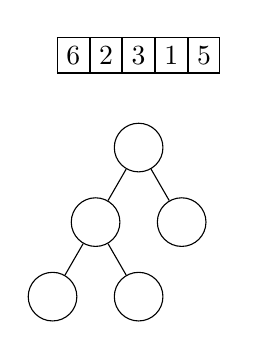
\begin{tikzpicture}[node distance=0.5cm and 0.1cm]
		\node (s) {\fbox{6}\fbox{2}\fbox{3}\fbox{1}\fbox{5}};
		\node[below =of s, circle, draw] (a) {\phantom{0}};
			\node[below left  =of a, circle, draw] (b) {\phantom{0}};
			\node[below right =of a, circle, draw] (c) {\phantom{0}};
			\node[below left  =of b, circle, draw] (d) {\phantom{0}};
			\node[below right =of b, circle, draw] (e) {\phantom{0}};
		\foreach \from/\to in {a/b,a/c,b/d,b/e}
			\draw (\from) -- (\to);
	\end{tikzpicture}
	\hspace{1 cm} \raisebox{1.5cm}{$\rightarrow$} \hspace{1 cm}
	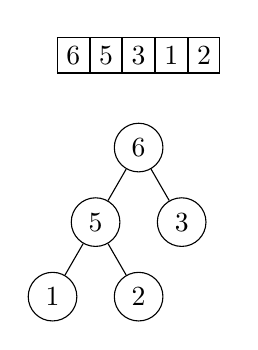
\begin{tikzpicture}[node distance=0.5cm and 0.1cm]
		\node (s) {\fbox{6}\fbox{5}\fbox{3}\fbox{1}\fbox{2}};
		\node[below =of s, circle, draw] (a) {6};
			\node[below left  =of a, circle, draw] (b) {5};
			\node[below right =of a, circle, draw] (c) {3};
			\node[below left  =of b, circle, draw] (d) {1};
			\node[below right =of b, circle, draw] (e) {2};
		\foreach \from/\to in {a/b,a/c,b/d,b/e}
			\draw (\from) -- (\to);
	\end{tikzpicture}
	\hspace{1 cm} \raisebox{1.5cm}{$\rightarrow$} \hspace{1 cm}
	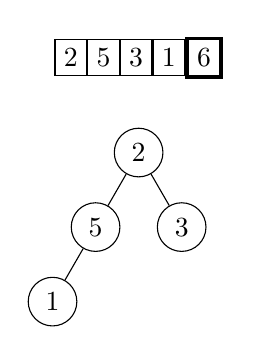
\begin{tikzpicture}[node distance=0.5cm and 0.1cm]
		\node (s) {\fbox{2}\fbox{5}\fbox{3}\fbox{1}\thickbox{6}};
		\node[below =of s, circle, draw] (a) {2};
			\node[below left  =of a, circle, draw] (b) {5};
			\node[below right =of a, circle, draw] (c) {3};
			\node[below left  =of b, circle, draw] (d) {1};
		\foreach \from/\to in {a/b,a/c,b/d}
			\draw (\from) -- (\to);
	\end{tikzpicture}
\end{figure}
\begin{figure}[h]
	\centering
	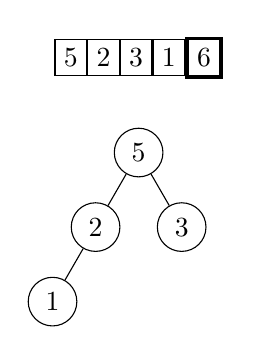
\begin{tikzpicture}[node distance=0.5cm and 0.1cm]
		\node (s) {\fbox{5}\fbox{2}\fbox{3}\fbox{1}\thickbox{6}};
		\node[below =of s, circle, draw] (a) {5};
			\node[below left  =of a, circle, draw] (b) {2};
			\node[below right =of a, circle, draw] (c) {3};
			\node[below left  =of b, circle, draw] (d) {1};
		\foreach \from/\to in {a/b,a/c,b/d}
			\draw (\from) -- (\to);
	\end{tikzpicture}
	\hspace{1 cm} \raisebox{1.5cm}{$\rightarrow$} \hspace{1 cm}
	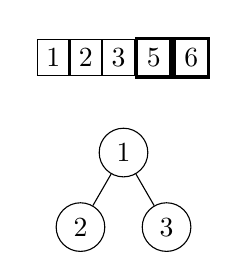
\begin{tikzpicture}[node distance=0.5cm and 0.1cm]
		\node (s) {\fbox{1}\fbox{2}\fbox{3}\thickbox{5}\thickbox{6}};
		\node[below =of s, circle, draw] (a) {1};
			\node[below left  =of a, circle, draw] (b) {2};
			\node[below right =of a, circle, draw] (c) {3};
		\foreach \from/\to in {a/b,a/c}
			\draw (\from) -- (\to);
	\end{tikzpicture}
	\hspace{1 cm} \raisebox{1.5cm}{$\rightarrow$} \hspace{1 cm}
	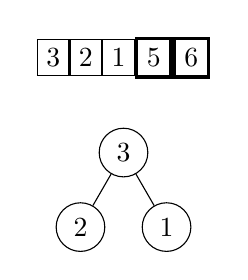
\begin{tikzpicture}[node distance=0.5cm and 0.1cm]
		\node (s) {\fbox{3}\fbox{2}\fbox{1}\thickbox{5}\thickbox{6}};
		\node[below =of s, circle, draw] (a) {3};
			\node[below left  =of a, circle, draw] (b) {2};
			\node[below right =of a, circle, draw] (c) {1};
		\foreach \from/\to in {a/b,a/c}
			\draw (\from) -- (\to);
	\end{tikzpicture}
\end{figure}


\clearpage
\section{Data Structures}

%-----------------------------------------------------------------------------------------------------------------

\subsection{Stacks}
\marginnote{\scriptsize{CLRS pg.232}}
A Stack is a dynamic set of data. It follows a {\bf Last-In First-Out} ordering system. Imagine a stack of plates, where you can only add to the stack and the top and only remove plates from the top. The data structure uses {\bf Push} to insert new data and {\bf Pop} to remove data. It uses a {\bf Top} pointer to keep track of the data structures position in memory.
\\ \\
Stacks are used ubiquitously. Used in algorithms in converting decimal numbers to binary, evaluating math expressions, maze back-tracking solutions. Most languages used stacks to resolve operations.
\begin{lstlisting}[style=pseudo]
function Push(x){
	S.top = S.top + 1
	S[S.top] = x
}

function Pop(){
	S.top = S.top - 1
	return S[S.top + 1]
}
\end{lstlisting}

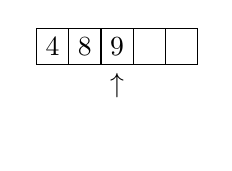
\begin{tikzpicture}[start chain=1 going right, node distance=-0.15mm]
	\node[draw, on chain=1] (a) {4};
	\node[draw, on chain=1] (b) {8};
	\node[draw, on chain=1] (c) {9};
	\node[draw, on chain=1] (d) {\phantom{0}};
	\node[draw, on chain=1] (e) {\phantom{0}};
	\node[below =of c] {$\uparrow$};
	\node at (0.8,-1.0)[text width=2.0cm] {\phantom{0}};
\end{tikzpicture}
\hspace{1 cm} \raisebox{0.5cm}{$\rightarrow$} \hspace{1 cm}
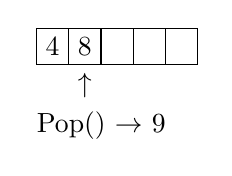
\begin{tikzpicture}[start chain=1 going right, node distance=-0.15mm]
	\node[draw, on chain=1] (a) {4};
	\node[draw, on chain=1] (b) {8};
	\node[draw, on chain=1] (c) {\phantom{0}};
	\node[draw, on chain=1] (d) {\phantom{0}};
	\node[draw, on chain=1] (e) {\phantom{0}};
	\node[below =of b] {$\uparrow$};
	\node at (0.8,-1.0)[text width=2.0cm] {Pop() $\rightarrow$ 9};
\end{tikzpicture}
\hspace{1 cm} \raisebox{0.5cm}{$\rightarrow$} \hspace{1 cm}
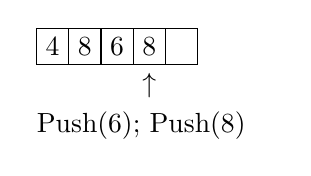
\begin{tikzpicture}[start chain=1 going right, node distance=-0.15mm]
	\node[draw, on chain=1] (a) {4};
	\node[draw, on chain=1] (b) {8};
	\node[draw, on chain=1] (c) {6};
	\node[draw, on chain=1] (d) {8};
	\node[draw, on chain=1] (e) {\phantom{0}};
	\node[below =of d] {$\uparrow$};
	\node at (1.3,-1.0)[text width=3.0cm] {Push(6); Push(8)};
\end{tikzpicture}


%-----------------------------------------------------------------------------------------------------------------

\subsection{Queues}
\marginnote{\scriptsize{CLRS pg.232}}
A Queue is a dynamic set of data. It follows a {\bf First-In First-Out} ordering system. Imagine a checkout at a store, you enter at the end of the queue and only leave at the front. The data structure uses {\bf Enqueue} to insert new data and {\bf Dequeue} to remove data. It uses a {\bf Head} and {\bf Tail} pointer to keep track of the data structures position in memory. To maximize memory use, queues are sometimes implemented cicular in nature
\\ \\
Queues are primarily used as {\bf Priority Queues}, where elements are added with a priority and removed in order of their priority. Many algorithms; including Dijkstra's, and A8 use priority queues to track the most efficient ways to solve their problem.
\begin{lstlisting}[style=pseudo]
function Enqueue(x){
	Q[Q.tail] = x
	if Q.tail == Q.length
		Q.tail = 1
	return Q.tail = Q.tail + 1
}

function Dequeue(){
	x = Q[Q.head]
	if Q.head == Q.length
		Q.head = 1
	else
		Q.head = Q.head + 1
	return x
}
\end{lstlisting}

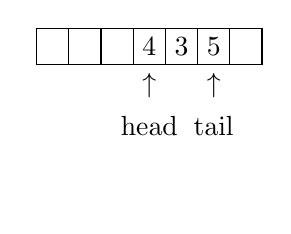
\begin{tikzpicture}[start chain=1 going right, node distance=-0.15mm]
	\node[draw, on chain=1] (f) {\phantom{0}};
	\node[draw, on chain=1] (g) {\phantom{0}};
	\node[draw, on chain=1] (a) {\phantom{0}};
	\node[draw, on chain=1] (b) {4};
	\node[draw, on chain=1] (c) {3};
	\node[draw, on chain=1] (d) {5};
	\node[draw, on chain=1] (e) {\phantom{0}};
	\node[below =of b] (head) {$\uparrow$};
		\node[below =of head] {head};
	\node[below =of d] (tail) {$\uparrow$};
		\node[below =of tail] {tail};
	\node at (0.8,-1.8)[text width=2.0cm] {\phantom{0}};
\end{tikzpicture}
\hspace{1 cm} \raisebox{0.8cm}{$\rightarrow$} \hspace{1 cm}
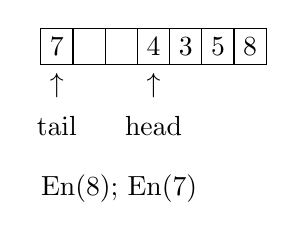
\begin{tikzpicture}[start chain=1 going right, node distance=-0.15mm]
	\node[draw, on chain=1] (f) {7};
	\node[draw, on chain=1] (g) {\phantom{0}};
	\node[draw, on chain=1] (a) {\phantom{0}};
	\node[draw, on chain=1] (b) {4};
	\node[draw, on chain=1] (c) {3};
	\node[draw, on chain=1] (d) {5};
	\node[draw, on chain=1] (e) {8};
	\node[below =of b] (head) {$\uparrow$};
		\node[below =of head] {head};
	\node[below =of f] (tail) {$\uparrow$};
		\node[below =of tail] {tail};
	\node at (0.8,-1.8)[text width=2.0cm] {En(8); En(7)};
\end{tikzpicture}
\hspace{1 cm} \raisebox{0.8cm}{$\rightarrow$} \hspace{1 cm}
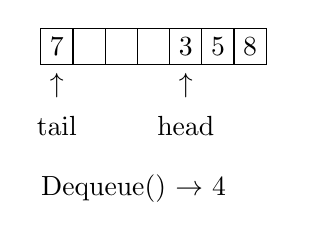
\begin{tikzpicture}[start chain=1 going right, node distance=-0.15mm]
	\node[draw, on chain=1] (f) {7};
	\node[draw, on chain=1] (g) {\phantom{0}};
	\node[draw, on chain=1] (a) {\phantom{0}};
	\node[draw, on chain=1] (b) {\phantom{0}};
	\node[draw, on chain=1] (c) {3};
	\node[draw, on chain=1] (d) {5};
	\node[draw, on chain=1] (e) {8};
	\node[below =of c] (head) {$\uparrow$};
		\node[below =of head] {head};
	\node[below =of f] (tail) {$\uparrow$};
		\node[below =of tail] {tail};
	\node at (1.3,-1.8)[text width=3.0cm] {Dequeue() $\rightarrow$ 4};
\end{tikzpicture}


%-----------------------------------------------------------------------------------------------------------------

\subsection{Linked Lists}
\marginnote{\scriptsize{CLRS pg.236}}
In Linked Lists data is stored linearly and sequenitially. Each node contains a pointer to the next node in the list. In a {\bf Double Linked List} each node also has a pointer to it's parent. Linked lists are better then dynamic arrays that their inserts and deletes always take constant time, and since it uses pointers, the data structure can be spread across memory. However, you can not random access a linked list, in order to get an element you must transverse the list to get there. Also linked lists use slightly more memory per node to track the pointers.

\begin{wrapfigure}{r}{7cm}
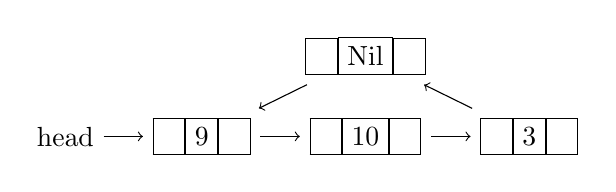
\begin{tikzpicture}[node distance=0.3cm and 0.5cm]
	\node (null)               {\fbox{\phantom{0}}\fbox{Nil}\fbox{\phantom{0}}};
	\node[below =of null] (e1) {\fbox{\phantom{0}}\fbox{10}\fbox{\phantom{0}}};
	\node[left =of e1] (e0)    {\fbox{\phantom{0}}\fbox{9}\fbox{\phantom{0}}};
	\node[right =of e1] (e2)   {\fbox{\phantom{0}}\fbox{3}\fbox{\phantom{0}}};
	\node[left =of e0] (head) {head};
	\foreach \from/\to in {null/e0, e0/e1,e1/e2,e2/null, head/e0}
		\draw[->] (\from) -- (\to);
\end{tikzpicture}
\end{wrapfigure}
\begin{lstlisting}[style=pseudo]
function Search(k){
	x = L.head
	while x != Nil && x.key != k
		x = x.next
	return x
}

function Insert(x){
	x.next = L.head
	if L.head != Nil
		L.head.prev = x
	L.head = x
	x.prev = Nil
}

function Delete(x){
	x.prev.next = x.next
	x.next.prev = x.prev
}
\end{lstlisting}



%-----------------------------------------------------------------------------------------------------------------

\subsection{Heaps}
\marginnote{\scriptsize{CLRS pg.151}}
Heaps are a datra structure which create a tree-like structure using sequential memory. They are defined by a {\bf Heap Property} which ditacte how the heap is formed, eg. max-heap property: Parent nodes are always larger then their children. The internal structure of a heap may be larger unordered, but the heap property ensures the top of the heap is the max element of the data structure. Heaps are useful for any scenerio where simply knowing the largest (or smallest) element is needed, eg. {\bf Priority Queues}. Using properties of sequiential access, node navigation can be done using math on the node's index.
\\ \\
Heapify ensures that the node at the given index is following the heap property, if not it will "float down" the data structure until it does. When extracting the max value from a heap, replace it with the last value in the heap, and Heapify from the top.

\begin{wrapfigure}{r}{4cm}
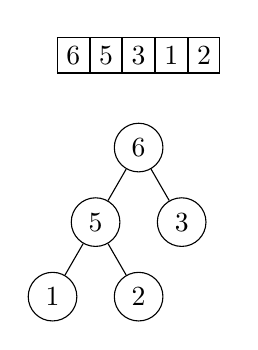
\begin{tikzpicture}[node distance=0.5cm and 0.1cm]
	\node (s) {\fbox{6}\fbox{5}\fbox{3}\fbox{1}\fbox{2}};
	\node[below =of s, circle, draw] (a) {6};
		\node[below left  =of a, circle, draw] (b) {5};
		\node[below right =of a, circle, draw] (c) {3};
		\node[below left  =of b, circle, draw] (d) {1};
		\node[below right =of b, circle, draw] (e) {2};
	\foreach \from/\to in {a/b,a/c,b/d,b/e}
		\draw (\from) -- (\to);
\end{tikzpicture}
\end{wrapfigure}

\begin{lstlisting}[style=pseudo]
Parent(i) => floor(i/2)
Left(i) => 2i
Right(i) => 2i + 1
function BuildHeap(A){
	for i = floor(A.length/2) -> 1
		Heapify(A, i)
}
function Heapify(A, i){
	if A[Left(i)] > A[i]
		largest = Left(i)
	else
		largest = i
	if A[Right(i)] > A[largest]
		largest = Right(i)
	if largest != i
		swap A[i] with A[largest]
		Heapify(A, largest)
}
function Extract(A){
	max = A[0]
	A[0] = A[A.length]
	Heapify(A,0)
	return max
}
\end{lstlisting}


%-----------------------------------------------------------------------------------------------------------------

\subsection{Hashtables}
\marginnote{\scriptsize{CLRS pg.257}}
Hashtables is a data structure that map keys to values in an associated array using a {\bf Hash Function}. A hash function should be choosen that limits clumping

A hash tables {\bf Load Factor} is the ratio of the number of elements in the data structure against it maximum size. When a hash table has a high load factor it has to be resized in order to avoid collisions. Resizing can be done one of two ways; {\bf Rebuilding} the entire hash table at once using a bigger size, or {\bf Incremental} where a new table is allocated, new values are only inserted into the new table, as well as moving over $n$ other elements from the old array. When the old table is empty it's removed from memory.

A technique to speed up deletes is to use {\bf Tombstones}. A tombstone is a special entry that is inserted in place of an element you wish to delete. It's ignored during lookups, and replaced during inserts.

Collisions resolution could be done one of several ways: {\bf Chaining}, {\bf Open Addressing}, {\bf Cuckoo}





%-----------------------------------------------------------------------------------------------------------------

\subsection{Binary Trees}
\marginnote{\scriptsize{CLRS pg.287}}
Binary Trees are family of data structures efficient at lookups. Data is stored that $Right \leq Node \leq Left$. BSTs are {\bf unbalanced}, meaning one part of the tree may become much larger then the other, hurting the efficiency. {\bf Search} and {\bf Insert} are $O(n \log n)$, {\bf Delete} is $O(n)$.

\begin{wrapfigure}{r}{4cm}
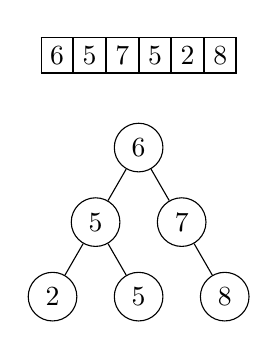
\begin{tikzpicture}[node distance=0.5cm and 0.1cm]
	\node (s) {\fbox{6}\fbox{5}\fbox{7}\fbox{5}\fbox{2}\fbox{8}};
	\node[below =of s, circle, draw] (a) {6};
		\node[below left  =of a, circle, draw] (b) {5};
		\node[below right =of a, circle, draw] (c) {7};
		\node[below left  =of b, circle, draw] (d) {2};
		\node[below right =of b, circle, draw] (e) {5};
		\node[below right =of c, circle, draw] (f) {8};
	\foreach \from/\to in {a/b,a/c,b/d,b/e,c/f}
		\draw (\from) -- (\to);
\end{tikzpicture}
\end{wrapfigure}

\begin{lstlisting}[style=pseudo]
function Search(node, val){
	if node == Nil or node.key == val
		return node
	if val > node.key
		return Search(node.left, val)
	else
		return Search(node.right, val)
}

//TODO: chage to recursive insert
function Insert(T, val){
	x = T.root
	while x != Nil
		if val > x.key
			x = x.left
		else
			x = x.right
	if val > x.parent.key
		x.left = val
	else
		x.right = val
}

function Delete(T, node){
	if node.left == Nil and node.right == Nil

}
\end{lstlisting}

%-----------------------------------------------------------------------------------------------------------------

\subsection{B-Trees}
\marginnote{\scriptsize{CLRS pg.488}}
B-Trees are an extreme form of {\bf k-ary Trees}, where k is very large. Each node has a minimum and maximum number of children it can have; $t-1$ and $2t - 1$ respectively, where $t$ is the {\bf order} of the tree. B-Trees are achieve extremely large tree structures with a small height when the order of the tree is high, number of nodes is $2t^h -1$ where $h$ is the height of the tree. This is very {\bf useful for when lookups are very expensive} and when lookups are best done in {\bf large sequiential blocks}. Mostly used for storing data on {\bf physical storage}.
\begin{figure}[h]
\centering
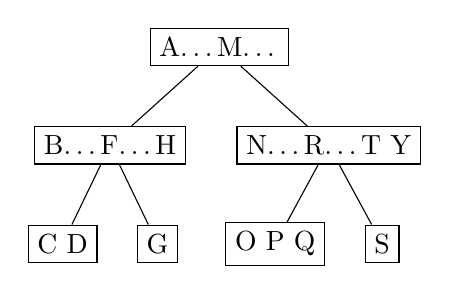
\begin{tikzpicture}[every tree node/.style={draw},
	level distance=1.25cm,sibling distance=.5cm,
	edge from parent path={(\tikzparentnode) -- (\tikzchildnode)}]
	\Tree [.{A\ldots M\ldots}
		[.{B\ldots F\ldots H}
			[.{C D} ]
			[.{G} ]
		]
		[.{N\ldots R\ldots T Y}
			[.{O P Q} ]
			[.{S} ]
		]
	]
\end{tikzpicture}
{\caption*{B-tree with order of 2}}
\end{figure}
\\
Inserting a node is slightly more complicated. When inserting a new value into a node that is full, we must split the node into smaller chunks. With deleting a value, you may have to rearrange a node's children.
\begin{figure}[h]
	\centering
	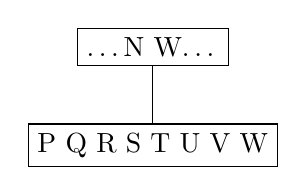
\begin{tikzpicture}[every tree node/.style={draw},
		level distance=1.25cm,sibling distance=.5cm,
		edge from parent path={(\tikzparentnode) -- (\tikzchildnode)}]
		\Tree [.{\ldots N W\ldots}
			[.{P Q R S T U V W} ]
		]
	\end{tikzpicture}
	\hspace{1 cm} \raisebox{1.0cm}{$\rightarrow$} \hspace{1 cm}
	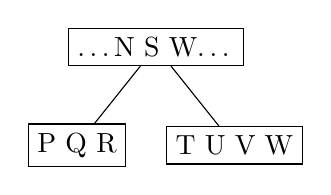
\begin{tikzpicture}[every tree node/.style={draw},
		level distance=1.25cm,sibling distance=.5cm,
		edge from parent path={(\tikzparentnode) -- (\tikzchildnode)}]
		\Tree [.{\ldots N S W\ldots}
			[.{P Q R} ]
			[.{T U V W} ]
		]
	\end{tikzpicture}
	{\caption*{Splitting a child node into 2 on $S$}}
\end{figure}


%-----------------------------------------------------------------------------------------------------------------

\subsection{Tries}
A Trie is an unique tree data structure, where a nodes location within the tree determines it's value. Each edge of the tree has a value given to it and as you traverse the tree to build the value of the node. Very useful for {\bf storing strings} and {\bf binary values}.
\\ \\
Tries have a {\bf faster worst case than hash tables} (no rebuilds), they can produce {\bf alpha-ordering} which may be useful for some applications like spell checking, and there is {\bf no chance for collisions}. However, Tries may need more memory, long entires can create useless nodes, and they require {\bf lots of random access memory} to operate. Tries are unique in that $Insert, Search, Delete \in O(M)$ where $M$ is the length of the longest node value.

\begin{figure}[h]
\centering
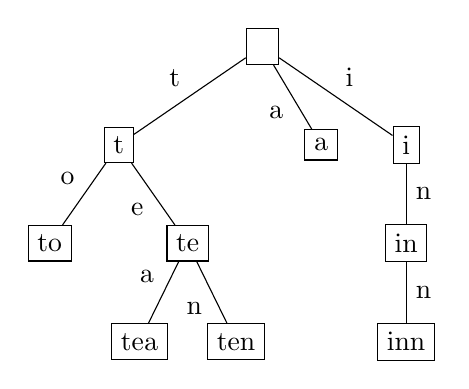
\begin{tikzpicture}[every tree node/.style={draw},
	level distance=1.25cm,sibling distance=.5cm,
	edge from parent path={(\tikzparentnode) -- (\tikzchildnode)}]
	\Tree [.\phantom{0}
		\edge node[auto=right] {t};
		[.t
			\edge node[auto=right] {o};
			[.to ]
			\edge node[auto=right] {e};
			[.te
				\edge node[auto=right] {a};
				[.tea ]
				\edge node[auto=right] {n};
				[.ten ]
			]
		]
		\edge node[auto=right] {a};
		[.a ]
		\edge node[auto=left] {i};
		[.i
			\edge node[auto=left] {n};
			[.in
				\edge node[auto=left] {n};
				[.inn ]
			]
		]
	]
\end{tikzpicture}
\end{figure}


%-----------------------------------------------------------------------------------------------------------------

\subsection{Radix Tree}
\marginnote{\scriptsize{CLRS pg.304}}
Radix Tress are space optimized {\bf Trie data strcutures} where each node with only one child is merged with it's parent, and it's edge is updated accordingly. They are much more efficient for small sets (especially if the strings are long) and for sets of strings that share long prefixes. $Insert, Search, Delete \in O(k)$ where $k$ is the length of the longest edge key.
\\ \\
Radix Trees are used in {\bf IP Routing}, where the ability to contain large ranges of values with a few exceptions is particularly suited to the hierarchical organization of IP addresses. They are useful for {\bf Inverted Indexes} in text documents for very fast searching through the document.
\begin{figure}[h]
\centering
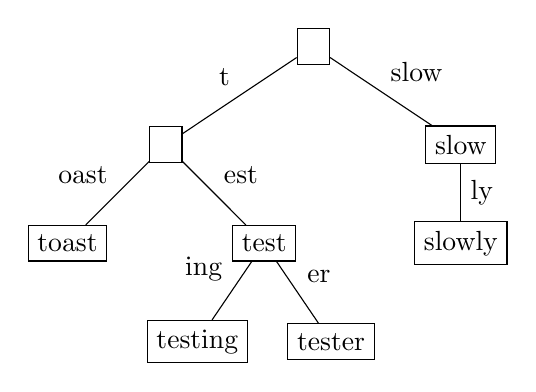
\begin{tikzpicture}[every tree node/.style={draw},
	level distance=1.25cm,sibling distance=.5cm,
	edge from parent path={(\tikzparentnode) -- (\tikzchildnode)}]
	\Tree [.\phantom{0}
		\edge node[auto=right] {t};
		[.\phantom{0}
			\edge node[auto=right] {oast};
			[.toast ]
			\edge node[auto=left] {est};
			[.test
				\edge node[auto=right] {ing};
				[.testing ]
				\edge node[auto=left] {er};
				[.tester ]
			]
		]
		\edge node[auto=left] {slow};
		[.slow
			\edge node[auto=left] {ly};
			[.slowly ]
		]
	]
\end{tikzpicture}
\end{figure}


%-----------------------------------------------------------------------------------------------------------------

\subsection{Self-Balancing Trees}
\marginnote{\scriptsize{CLRS pg.308}}

A Self-Balancing Tree is a binary search tree that automatically keeps its height small during inserts and deletes. The time it takes for an operation on aBinary Search Tree is dependant on it's height, which in extreme cases can result in long and unexpected run times. Self-Balancing Trees attempt to correct this by using {\bf Tree Rotations} to maintain tree properties that ensure a predictable height of the tree. Whenever a node is inserted or deleted, we need to check the node's children for consistency of the height property. Search, Insert, and Deletes all take $O(\log n)$ time in both the average and worst cases. The two most common Self-Balancing Trees are {\bf AVL Trees} and {\bf Red-Black Trees}.

\begin{figure}[h]
\centering
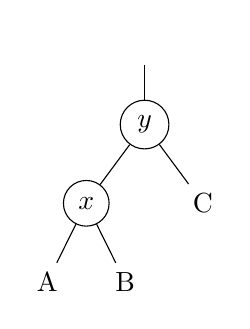
\begin{tikzpicture}[
		every tree node/.style={},
		level distance=1.0cm,sibling distance=.5cm,
		edge from parent path={(\tikzparentnode) -- (\tikzchildnode)}
	]
	\Tree [.\phantom{0}
		[.\node[draw, circle] {$y$};
			[.\node[draw, circle] {$x$};
				[.A ]
				[.B ]
			]
			[.C ]
		]
	]
\end{tikzpicture}
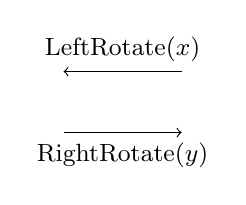
\begin{tikzpicture}[node distance=0.3cm and 1.5cm]
	\node                (tl) {\phantom{0}};
	\node [right =of tl] (tr) {\phantom{0}};
	\node [below =of tl] (bl) {\phantom{0}};
	\node [right =of bl] (br) {\phantom{0}};

	\draw[->] (tr) --(tl) node[above,midway] {\small LeftRotate($x$)};
	\draw[->] (bl) --(br) node[below,midway] {\small RightRotate($y$)};

\end{tikzpicture}
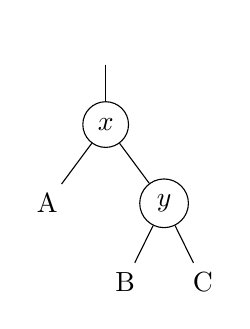
\begin{tikzpicture}[
		every tree node/.style={},
		level distance=1.0cm,sibling distance=.5cm,
		edge from parent path={(\tikzparentnode) -- (\tikzchildnode)}
	]
	\Tree [.\phantom{0}
		[.\node[draw, circle] {$x$};
			[.A ]
			[.\node[draw, circle] {$y$};
				[.B ]
				[.C ]
			]
		]
	]
\end{tikzpicture}
%{\caption*{Basic Tree Rotations}}
\end{figure}

%-----------------------------------------------------------------------------------------------------------------

\subsubsection{AVL Trees}
The height property of an AVL Tree is that {\bf the heights of the two child subtrees of any node differ by at most one}. AVL Trees are more rigidly balanced than Red-Black Trees, leading to {\bf slower inserts and deletes} but {\bf faster search}.

\begin{minipage}{\linewidth}
\begin{lstlisting}[style=pseudo]
function balanceFactor(node) => height(node.left) - height(node.right)
function Insert(node, val){
	if node is Nil
		node.key = val
		return node
	if val > node.key
		node.left = Insert(node.left, val)
		if balanceFactor(node) > 1
			if val > node.left.key
				LeftRotate(node)
			LeftRotate(node)
	if val <= node.key
		node.right = Insert(node.right, val)
		if balanceFactor(node) < -1
			if val < node.right.key
				RightRotate(node)
			RightRotate(node)
	return node
}

function Delete(z){
	//finish later, very complex
}
\end{lstlisting}
\end{minipage}
%-----------------------------------------------------------------------------------------------------------------

\subsubsection{Red-Black Trees}
Red-Black Trees are less rigidly balanced than AVL Trees, leading to {\bf slower search} but {\bf faster inserts and deletes}. The height properties of a Red-Black Tree are as follows:
\begin{enumerate}
	\item A node may be red or black
	\item All leaves are black
	\item Every red node must have two black child nodes
	\item Every path from the root to a leaf must have the same number of black nodes.
\end{enumerate}

\begin{figure}[h]
\centering
\tikzset{
	node_black/.style = {
		circle, white, font=\sffamily\bfseries, draw=black, fill=black
	},
	node_red/.style = {
		circle, red, draw=red, very thick
	},
	node_nil/.style = {
		white, font=\scriptsize\sffamily\bfseries, draw=black, fill=black
	}
}
\begin{tikzpicture}[every tree node/.style={draw},
	level distance=1.25cm,sibling distance=.5cm,
	edge from parent path={(\tikzparentnode) -- (\tikzchildnode)}]
	\Tree [.\node[node_black] {13};
		[.\node[node_red] {8};
			[.\node[node_black] {1};
				[.\node[node_nil] {NIL}; ]
				[.\node[node_red] {6};
					[.\node[node_nil] {NIL}; ]
				]
			]
			[.\node[node_black] {11};
				[.\node[node_nil] {NIL}; ]
				[.\node[node_nil] {NIL}; ]
			]
		]
		[.\node[node_red] {17};
			[.\node[node_black] {15};
				[.\node[node_nil] {NIL}; ]
				[.\node[node_nil] {NIL}; ]
			]
			[.\node[node_black] {25};
				[.\node[node_red] {22};
					[.\node[node_nil] {NIL}; ]
					[.\node[node_nil] {NIL}; ]
				]
				[.\node[node_red] {27};
					[.\node[node_nil] {NIL}; ]
					[.\node[node_nil] {NIL}; ]
				]
			]
		]
	]
\end{tikzpicture}
\end{figure}

\begin{minipage}{\linewidth}
\begin{lstlisting}[style=pseudo]
//TODO: Make recursive
function Insert(z){
	find leaf where node should be attached -> y
	z.parent = y
	if z.key > y.key
		y.left = z
	else
		y.right = z
	z.color = red

	//Maintain height property
	while z.parent is red
		if z.parent is a left-child
			if z.uncle is red
				z.parent.color = black
				z.uncle.color = black
				z.grandparent.color = red
				z = z.grandparent
			if z.uncle is black and z is a right-child
				z = z.parent
				LeftRotate(z)
			if z's uncle is black and z is a left-child
				z.parent.color = black
				z.grandparent.color = red
				RightRotate(z.grandparent)
		else
			Same as above but switch left and right rotate
	root.color = black
}

function Delete(z){
	//finish later, very complex
}
\end{lstlisting}
\end{minipage}




%-----------------------------------------------------------------------------------------------------------------

\subsection{Bloom Filter}
A Bloom Filter is a space efficient probalistic data structure that's used to test whether an element is in a set. False positives are possible, but {\bf false negatives} are not. An empty Bloom Filter is a bit array of $m$ bits all set to 0. Whenever you add an element to the set use $k$ hash functions and flip all the corresponing entires to 1. To test if an entry belongs to the set, simply hash it and check the corresponding bit entires. If any of them are 0 the element is not part of the set. The probability of a {\bf false positive} is $(1 - e^{-kn/m})^k$, where $n$ is the number of elements encoded in the set.
\\ \\
Bloom Filters are used in Chrome to detect bad urls from a list, in BigTable to remove unnecessary table lookups, and in url shortners.

\begin{figure}[h]
	\centering
	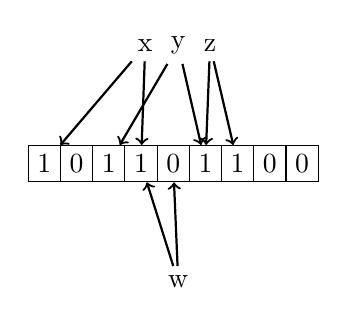
\begin{tikzpicture}[start chain=1 going right, node distance=-0.15mm]
		\node (y) {y};
		\node[left =of y] (x) {x};
		\node[right =of y] (z) {z};
		\node[draw, on chain=1] at (-1.7,-1.5) (a) {1};
		\node[draw, on chain=1] (b) {0};
		\node[draw, on chain=1] (c) {1};
		\node[draw, on chain=1] (d) {1};
		\node[draw, on chain=1] (e) {0};
		\node[draw, on chain=1] (f) {1};
		\node[draw, on chain=1] (g) {1};
		\node[draw, on chain=1] (h) {0};
		\node[draw, on chain=1] (i) {0};
		\node at (0,-3.0) (w) {w};
		\foreach \from/\to in {x/a,x/d,y/c,y/f,z/f,z/g,w/d,w/e}
			\draw[->, thick] (\from) -- (\to);
	\end{tikzpicture}
	{\caption*{$x$, $y$, $z$ are in the set, where $w$ is not}}
\end{figure}

\clearpage
\section{Graph Algorithms}
%-----------------------------------------------------------------------------------------------------------------
	\subsection{Representation}
	\marginnote{\scriptsize{CLRS pg.308}}
	A graph can either be directed or undirected. {\bf Undirected Graphs} simply have links betwen two nodes, where {\bf Directed Graphs} have one-way links between nodes. We can represent a graph in one of two ways; Adjacency Lists and Adjacency Matricies. {\bf Adjacency Lists} are useful for when the graph is {\bf sparse}, few edges compared to nodes. {\bf Adjacency Matricies} are useful for when the graph is {\bf dense}, many edges compared to nodes.
	\begin{figure}[h]
		\centering
		\begin{minipage}[b][4cm][b]{.3\textwidth}
			\centering
			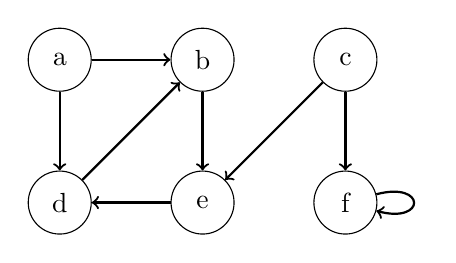
\begin{tikzpicture}[
					every node/.style={draw, circle},
					minimum size=0.8cm,
					every loop/.style={},
					node distance=1.0cm and 1.0cm]
				\node[]            (a) {a};
				\node[right =of a] (b) {b};
				\node[right =of b] (c) {c};
				\node[below =of a] (d) {d};
				\node[right =of d] (e) {e};
				\node[right =of e] (f) {f};
				\foreach \from/\to in {a/b, a/d, b/e, c/e, c/f, d/b, e/d}
					\draw[->, thick] (\from) -- (\to);
				\draw[->, thick] (f) to[loop right] (f);
			\end{tikzpicture}
			{\caption*{Directed Graph}}
		\end{minipage}
		\begin{minipage}[b][4cm][b]{.3\textwidth}
			\centering
			$a \rightarrow b,d$            \\
			$b \rightarrow e \phantom{,a}$ \\
			$c \rightarrow e,f$            \\
			$d \rightarrow b \phantom{,a}$ \\
			$e \rightarrow d \phantom{,a}$ \\
			$f \rightarrow f \phantom{,a}$
			{\caption*{Adjacency List}}
		\end{minipage}
		\begin{minipage}[b][4cm][b]{.3\textwidth}
			\centering
			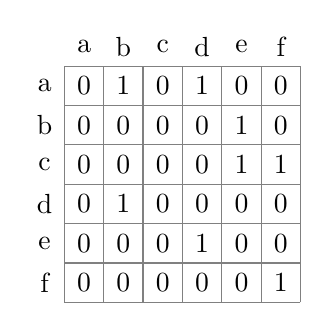
\begin{tikzpicture}
				\draw[step=0.5cm,color=gray] (-1.5,-1.5) grid (1.5,1.5);
				\foreach \v [count=\i] in {
					\phantom{0},a,b,c,d,e,f,
					a,0,1,0,1,0,0,
					b,0,0,0,0,1,0,
					c,0,0,0,0,1,1,
					d,0,1,0,0,0,0,
					e,0,0,0,1,0,0,
					f,0,0,0,0,0,1}{
				\draw let
					\n0 = 7,
					\n1 = {int(mod(\i-1,\n0))},
					\n2 = {-2.0 + 0.25 + \n1 * 0.5},
					\n3 = {2.0 + int((\i-1)/-\n0) * 0.5 - 0.25}
				in node at (\n2, \n3) {\v};
				}
			\end{tikzpicture}
			{\caption*{Adjacency Matrix}}
		\end{minipage}
	\end{figure}


	%-----------------------------------------------------------------------------------------------------------------

	\subsection{Breadth First Search}
	\marginnote{\scriptsize{CLRS pg.594}}
	Breadth-First Search is a strategy for searching a graph. It's starts at the root node, visits all of it's neighbours, then each of them, visits their neighbours. As it runs it produces a {\bf Breadth-First Tree}, where the depth of the tree indicates how far apart the root and that node is in the graph.
	\\ \\
	{\bf Aux. Space} is $\Omega(V + E)$ using an Adj. List and $\Omega(V^2)$ using an Adj. Matrix. {\bf Worst Case Complexity} is $O(V + E)$, where $O(E)$ may vary between $O(V)$ and $O(V^2)$ depending on how dense the graph is. Used for {\bf finding the shortest path} between nodes and asserting if two nodes are connected to eachother.

	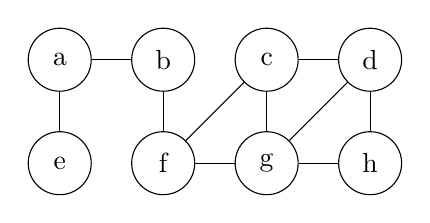
\begin{tikzpicture}[
			every node/.style={draw, circle},
			minimum size=0.8cm,
			node distance=0.5cm and 0.5cm]
		\node[]            (a) {a};
		\node[right =of a] (b) {b};
		\node[right =of b] (c) {c};
		\node[right =of c] (d) {d};

		\node[below =of a] (e) {e};
		\node[right =of e] (f) {f};
		\node[right =of f] (g) {g};
		\node[right =of g] (h) {h};
		\foreach \from/\to in {a/b, a/e, b/f, f/c, f/g, c/d, g/h,
								c/g,g/d,d/h}
			\draw (\from) -- (\to);
	\end{tikzpicture}
	\hspace{0.5 cm} \raisebox{1.0cm}{$\rightarrow$} \hspace{0.5 cm}
	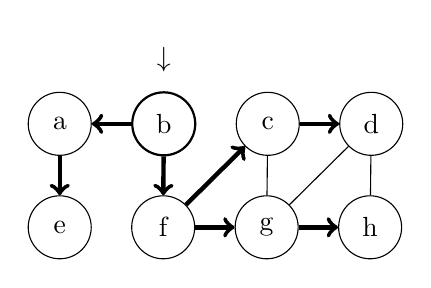
\begin{tikzpicture}[
			every node/.style={draw, circle},
			minimum size=0.8cm,
			node distance=0.5cm and 0.5cm]
		\node[]            (a) {a};
		\node[right =of a, label=above:$\downarrow$, thick] (b) {b};
		\node[right =of b] (c) {c};
		\node[right =of c] (d) {d};

		\node[below =of a] (e) {e};
		\node[right =of e] (f) {f};
		\node[right =of f] (g) {g};
		\node[right =of g] (h) {h};
		\foreach \from/\to in {b/a, a/e, b/f, f/c, f/g, c/d, g/h}
			\draw[->, ultra thick] (\from) -- (\to);
		\foreach \from/\to in {c/g,g/d,d/h}
			\draw (\from) -- (\to);
	\end{tikzpicture}
	\hspace{0.5 cm} \raisebox{1.0cm}{$\rightarrow$} \hspace{0.5 cm}
	\begin{tikzpicture}[every tree node/.style={},
		level distance=0.75cm,sibling distance=.5cm,
		edge from parent path={(\tikzparentnode) -- (\tikzchildnode)}]
		\Tree [.b
			[.a
				[.e ]
			]
			[.f
				[.c
					[.d ]
				]
				[.g
					[.h ]
				]
			]
		]
	\end{tikzpicture}

	\begin{lstlisting}[style=pseudo]
	BFS(start, goal){
		create queue Q
		create list R
		Q.enqueue(start)
		R.push(start)

		while Q is not empty
			t = Q.dequeue()
			t.visited = true
			if t is goal
				return R
			for all neighbours v of t
				if v is not in R || v.visited == false
					v.visited = true
					R.push(v)
					Q.enqueue(v)
	}
	\end{lstlisting}





	%-----------------------------------------------------------------------------------------------------------------

	\subsection{Depth First Search}
	\marginnote{\scriptsize{CLRS pg.603}}
	Depth-First Search is a strategy for searching a graph. It's starts at the root node and explores as deep as possible before backtracking. By tracking and applying a {\bf timestamp} (increments once a node has been visitied) to each node as it's visited for the first and last time, you can sort the nodes by {\bf preorder} and {\bf postorder}, respectively. Postordering the nodes provides you with a {\bf Topological Sort} of the graph.
	\\ \\
	Used in AI for limiting the depth of decisions trees and evaluating branches based on heurstics, maze generation, and topological sorting.

	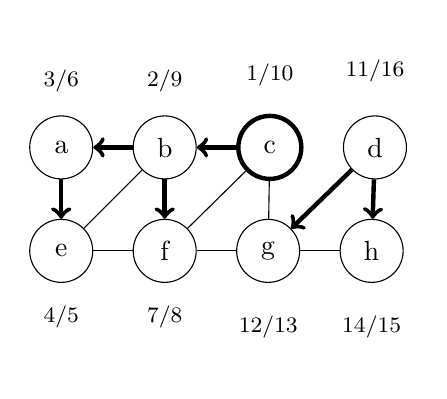
\begin{tikzpicture}[
			every node/.style={draw, circle},
			minimum size=0.8cm,
			node distance=0.5cm and 0.5cm]
		\node[             label=above:\footnotesize 3/6]   (a) {a};
		\node[right =of a, label=above:\footnotesize 2/9]   (b) {b};
		\node[right =of b, label=above:\footnotesize 1/10, ultra thick]  (c) {c};
		\node[right =of c, label=above:\footnotesize 11/16] (d) {d};

		\node[below =of a, label=below:\footnotesize 4/5]  (e) {e};
		\node[right =of e, label=below:\footnotesize 7/8]   (f) {f};
		\node[right =of f, label=below:\footnotesize 12/13] (g) {g};
		\node[right =of g, label=below:\footnotesize 14/15] (h) {h};
		\foreach \from/\to in {a/e, b/a, b/f, c/b, d/g, d/h}
			\draw[->, ultra thick] (\from) -- (\to);
		\foreach \from/\to in {c/f, e/b, f/e, g/f, g/c, h/g}
			\draw (\from) -- (\to);
	\end{tikzpicture}
	\hspace{2cm}
	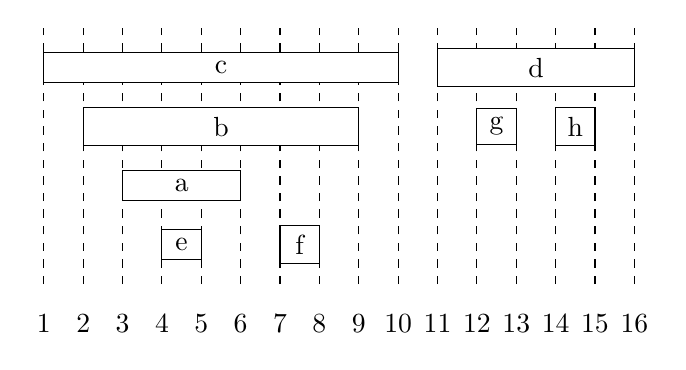
\begin{tikzpicture}[every node/.style={fill=white}]
		\foreach \i in {1,...,16} {
			\draw [dashed] (\i*0.5,1) -- (\i*.5,4.25);
			\node at (\i*0.5,0.5) {\i};
		}
		\foreach \t/\s/\e/\h in {
			a/3/6/2,
			b/2/9/1,
			c/1/10/0,
			d/11/16/0,
			e/4/5/3,
			f/7/8/3,
			g/12/13/1,
			h/14/15/1}{
			\draw let
				\n0 = {int(\e - \s)/2}, % half width
				\n1 = {\n0/2 + \s/2} %relative x to width
			in node[draw, minimum width=\n0cm] at (\n1, 3.75 - \h*0.75) {\t};
		}
	\end{tikzpicture}

	\begin{lstlisting}[style=pseudo]
	DFS(start){
		create stack S
		S.push(start)
		timestamp = 0
		while S is not empty
			node = S.pop()
			node.begin = timestamp
			for all neighbours v of node
				if v.visited == false
					S.push(v)
			timestamp = timestamp + 1
			node.visited = true
			node.end = timestamp
	}
	\end{lstlisting}


	%-----------------------------------------------------------------------------------------------------------------

	\subsection{Topological Sort}
	\marginnote{\scriptsize{CLRS pg.613}}
	The Toplogical Sort of a {\bf directed graph} is a linear ordering of the nodes, such that every node comes before the node it's connected to. An example is that if each node is a task and the edges between nodes represent constriants on finishing tasks before starting another, topologically sorting this graph would ensure an order to complete the tasks which would provide no conflicts.
	\\ \\
	Topological Sort is a modified Depth-First Search alogithm, where we {\bf postorder} the nodes, or sort the descending by the last when they were visited.

	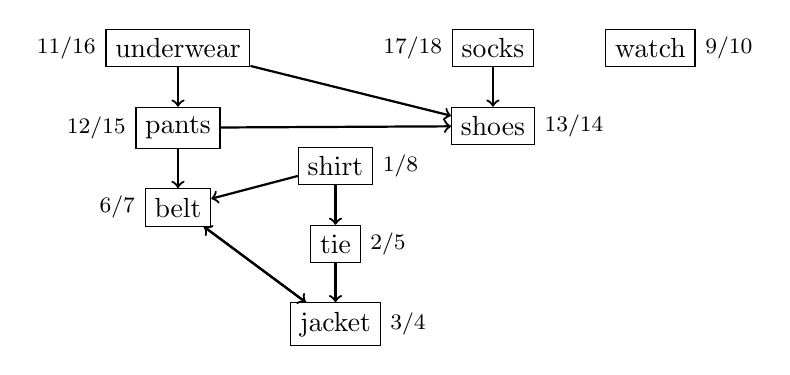
\begin{tikzpicture}[node distance=0.5cm and 0.8cm, every node/.style={draw}]
		\node[label=left:\footnotesize  11/16] (underwear) {underwear};
		\node[label=left:\footnotesize  12/15, below =of underwear] (pants) {pants};
		\node[label=left:\footnotesize  6/7, below =of pants] (belt) {belt};
		\node[label=right:\footnotesize 1/8] at (2, -1.5) (shirt) {shirt};
		\node[label=right:\footnotesize 2/5, below =of shirt] (tie) {tie};
		\node[label=right:\footnotesize 3/4, below =of tie] (jacket) {jacket};
		\node[label=left:\footnotesize  17/18] at (4,0) (socks) {socks};
		\node[label=right:\footnotesize 13/14, below =of socks] (shoes) {shoes};
		\node[label=right:\footnotesize 9/10] at (6,0) (watch) {watch};

		\foreach \from/\to in {
			underwear/pants, underwear/shoes, pants/shoes, socks/shoes,
			pants/belt, belt/jacket, shirt/belt, shirt/tie, tie/jacket, jacket/belt}
			\draw[->, thick] (\from) -- (\to);
	\end{tikzpicture}

	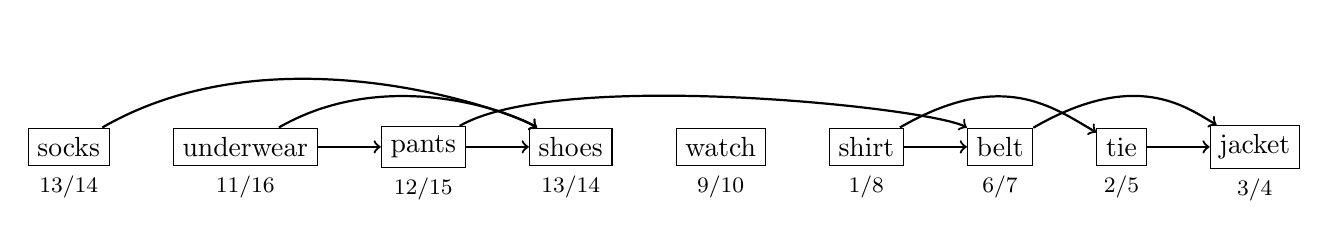
\begin{tikzpicture}[node distance=0.5cm and 0.8cm, every node/.style={draw}]
		\node[label=below:\footnotesize 13/14]  (socks) {socks};
		\node[label=below:\footnotesize 11/16, right =of socks] (underwear) {underwear};
		\node[label=below:\footnotesize 12/15, right =of underwear] (pants) {pants};
		\node[label=below:\footnotesize 13/14, right =of pants] (shoes) {shoes};
		\node[label=below:\footnotesize 9/10, right =of shoes] (watch) {watch};
		\node[label=below:\footnotesize 1/8, right =of watch] (shirt) {shirt};
		\node[label=below:\footnotesize 6/7, right =of shirt] (belt) {belt};
		\node[label=below:\footnotesize 2/5, right =of belt] (tie) {tie};
		\node[label=below:\footnotesize 3/4, right =of tie] (jacket) {jacket};
		\foreach \from/\to in {underwear/pants, pants/shoes,shirt/belt, tie/jacket}
			\draw[->, thick] (\from) -- (\to);
		\draw[->, thick] (socks)     .. controls +(30:3cm) and +(150:1cm) .. (shoes);
		\draw[->, thick] (underwear) .. controls +(30:2cm) and +(150:1cm) .. (shoes);
		\draw[->, thick] (shirt)     .. controls +(30:2cm) and +(150:1cm) .. (tie);
		\draw[->, thick] (belt)      .. controls +(30:2cm) and +(150:1cm) .. (jacket);
		\draw[->, thick] (pants)     .. controls +(30:2cm) and +(150:1cm) .. (belt);
	\end{tikzpicture}



	%-----------------------------------------------------------------------------------------------------------------

	\subsection{Minimum Spanning Tree}
	\marginnote{\scriptsize{CLRS pg.625}}
	A Minimum Spanning Tree is a subgraph of a graph that contains all nodes and has lowest combined weight of all of it's edges. It's possible to have multiple Minimum Spanning Trees per graph, if the edge weights are not unique.

	\begin{figure}[h]
		\centering
		\tikzstyle{vertex}=[draw,circle,minimum size=0.8cm]
		\tikzstyle{edge} = [draw,-]
		\tikzstyle{selected edge} = [draw,ultra thick,-]
		\begin{tikzpicture}[auto, swap]
			\foreach \pos/\name in {{(0,2)/a}, {(2,1)/b}, {(4,1)/c},
									{(0,0)/d}, {(3,0)/e}, {(2,-1)/f}, {(4,-1)/g}}
				\node[vertex] (\name) at \pos {$\name$};
			\foreach \source/ \dest /\weight in {b/a/7, c/b/8,d/a/5,d/b/9,
												 e/b/7, e/c/5,e/d/15,
												 f/d/6,f/e/8,
												 g/e/9,g/f/11}
				\path[edge] (\source) -- node {\scriptsize $\weight$} (\dest);
			\foreach \source / \dest in {d/a,d/f,a/b,b/e,e/c,e/g}
				\path [selected edge] (\source) -- (\dest);
		\end{tikzpicture}
		{\caption*{Minimum Spanning Tree of a weighted graph}}
	\end{figure}

	\subsubsection{Prim's Alogithm}
	\marginnote{\scriptsize{CLRS pg.634}}
	Prim's Alogithm is a {\bf Greedy Algorithm} using {\bf Priority Queues}. It's running time is $O(E + V \log V)$ and best used for {\bf dense graphs}. At each step it grows the tree by one node, selecting the smallest edge available.

	\begin{lstlisting}[style=pseudo]
	PrimMST(G){
		add all nodes in G to Queue, Q with key = \infty
		while Q is not empty
			x = Q.extractMin()
			for all neighbours v of x
				if v is in Q and weight(x,v) < v.key
					v.parent = x
					v.key = weight(x,v)
	}
	\end{lstlisting}


	\subsubsection{Krushal's Alogithm}
	\marginnote{\scriptsize{CLRS pg.631}}
	Krushal's Alogithm is a {\bf Greedy Algorithm} using {\bf Disjoint Sets}. It's running time is $O(E \log V)$ and best used for {\bf sparse graphs}. It first creates a set for each node, and then a set of all edges ordered by weight. For each edge, if both nodes aren't in the same set together, it merges them together and adds that edge to the solution

	\begin{lstlisting}[style=pseudo]
	KrushalMST(G){
		make Result an empty set
		make a set for each node that contains it
		foreach (u, v) in G.Edges ordered by weight(u, v)
			if Find-Set(u) != Find-Set(v)
				add (u,v) to Result
				Join-Sets(u, v)
		return Result
	}
	\end{lstlisting}


	%-----------------------------------------------------------------------------------------------------------------

	\subsection{Dijsktra's Algorithm}
	\marginnote{\scriptsize{CLRS pg.658}}

	Dijsktra's Algorithm finds the shortest path in a weighted graph from a single source. As Dijsktra's Algorithm tranverses the graph, it follows the path of lowest expected total distance. It keeps track of "how good" each branch is using a {\bf Min-Priority Queue}. It uses a greedy algorithm to choose the next node for each branch and will switch to a different branch if it no longer is the fastest. The variable $distance$ on each node in our code tracks the shortest path value to get to that node from the start.
	\\ \\
	It's running time is $O(E + V \log V)$.

	\begin{lstlisting}[style=pseudo]
	Dijsktra(G, start, goal){
		create Priority Queue Q
		add all nodes to Q with distance of \infty
		start.distance = 0
		while Q is not empty
			current = Q.extractMin()
			if current is goal
				goal.parent = current
				return ReconstructPath(goal, empty list)
			for each neighbour of current
				temp = current.distance + weight(current, neighbour)
				if temp < neighbour.distance
					neighbour.distance = temp
					neighbour.parent = current
	}
	ReconstructPath(node, result){
		if node has parent
			ReconstructPath(node.parent, result)
		result.push(node)
		return result
	}
	\end{lstlisting}


	%-----------------------------------------------------------------------------------------------------------------

	\subsection{A*}
	\marginnote{\scriptsize{CLRS pg.308}}
	The A* algorithm is a generalization of Dijkstra's algorithm that cuts down on the size of the subgraph that must be explored by using an additional {\bf heuristic} unique to the problem. The heuristic function helps guide the path in which the algorithm takes next. For example if the nodes have a coordinate location, the heuristic function could be the euclidean distance between the current node and the goal, making sure that the algorithm tries the closer node first.
	\\ \\
	Running time is $O(\log h^{*}(x))$, where $h^{*}(x)$ is the optimal heuristic function.

	\begin{lstlisting}[style=pseudo]
	Dijsktra(G, start, goal){
		create Priority Queue Q
		add all nodes to Q with score of \infty
		start.score = 0
		while Q is not empty
			current = Q.extractMin()
			if current is goal
				goal.parent = current
				return ReconstructPath(goal, empty list)
			for each neighbour of current
				temp = current.score + weight(current, neighbour) + heuristic(neighbor, goal)
				if temp < neighbour.score
					neighbour.score = temp
					neighbour.parent = current
	}
	ReconstructPath(node, result){
		if node has parent
			ReconstructPath(node.parent, result)
		result.push(node)
		return result
	}
	\end{lstlisting}


	%-----------------------------------------------------------------------------------------------------------------

	\subsection{k-Means Clustering}
	\marginnote{\scriptsize{CLRS pg.308}}
	%-----------------------------------------------------------------------------------------------------------------

	\subsection{Convex Hull}
	\marginnote{\scriptsize{CLRS pg.1029}}
	The Convex Hull of a set of points is the smallest polygon that contains all the points. Think of it like an elastic band wrapped around a number of pegs in a board. Used with bezier curves, pattern recogintion, image processing, statistics, and static code analysis.

		\subsubsection{Graham's Scan}
		Graham's Scan starts at the lowest point in the set and iterates over the points in a counterclockwise direction, relative to this point. At each step it calculates the angle between the last three points, if that angle is towards the left, we remove the last two points and try other ones. Running time of $O(n \log n)$

		\begin{lstlisting}[style=pseudo]
		GScan(P){
			root = lowest point in P
			S = all points in P sorted by relative angle to root
			Hull = empty list

			Hull.push(root)
			Hull.push(S.pop())

			while S is not empty
				next = S.top()
				if angleDirection(Hull.secondLast(), Hull.last(), next) is left
					Hull.push(S.pop())
				else
					Hull.pop()
			return Hull
		}
		\end{lstlisting}

		\tikzstyle{point}=[circle,fill=black,minimum size=0.15cm,inner sep=0pt]
		\begin{tikzpicture}
			\node[point, label=below:\scriptsize p0] (p0) at (-1,-2) {};
			\foreach \pos/\name in {{(4,-1)/p1}, {(2,-1)/p2}, {(3,0)/p3}, {(4,1.5)/p4}, {(2,1)/p5}, {(0,0)/p6}, {(0,2)/p7}} {
				\node[point] (\name) at \pos {};
				\node[anchor=south west] at (\name) {\scriptsize \name};
			}
			\foreach \name in {p1,p2,p3,p4,p5,p6,p7}
				\path[draw, dotted, thick] (p0) -- (\name);

			\path[draw, ultra thick] (p0) -- (p1);
			\path[draw] (p1) -- (p2);

			\coordinate (b) at (-1,-2);
			\coordinate (c) at (4,-1);
			\coordinate (a) at (2,-1);
			\draw[fill=black!20] (c) -- ($(c)!8mm!(b)$) to[bend left] ($(c)!8mm!(a)$)  -- cycle;
		\end{tikzpicture}
		\hspace{2cm}
		\begin{tikzpicture}
			\coordinate (a) at (4,-1);
			\coordinate (c) at (2,-1);
			\coordinate (b) at (3,0);
			\draw[fill=black!20] (c) -- ($(c)!8mm!(b)$) to[bend left] ($(c)!8mm!(a)$)  -- cycle;

			\node[point, label=below:\scriptsize p0] (p0) at (-1,-2) {};
			\foreach \pos/\name in {{(4,-1)/p1}, {(2,-1)/p2}, {(3,0)/p3}, {(4,1.5)/p4}, {(2,1)/p5}, {(0,0)/p6}, {(0,2)/p7}} {
				\node[point] (\name) at \pos {};
				\node[anchor=south west] at (\name) {\scriptsize \name};
			}
			\foreach \name in {p1,p2,p3,p4,p5,p6,p7}
				\path[draw, dotted, thick] (p0) -- (\name);

			\path[draw, ultra thick] (p0) -- (p1);
			\path[draw, ultra thick] (p1) -- (p2);
			\path[draw] (p2) -- (p3);
		\end{tikzpicture}

		\begin{tikzpicture}
			\node[point, label=below:\scriptsize p0] (p0) at (-1,-2) {};
			\foreach \pos/\name in {{(4,-1)/p1}, {(2,-1)/p2}, {(3,0)/p3}, {(4,1.5)/p4}, {(2,1)/p5}, {(0,0)/p6}, {(0,2)/p7}} {
				\node[point] (\name) at \pos {};
				\node[anchor=south west] at (\name) {\scriptsize \name};
			}
			\foreach \name in {p1,p2,p3,p4,p5,p6,p7}
				\path[draw, dotted, thick] (p0) -- (\name);

			\path[draw, ultra thick] (p0) -- (p1);
			\path[draw] (p1) -- (p3);

			\coordinate (b) at (-1,-2);
			\coordinate (c) at (4,-1);
			\coordinate (a) at (3,0);
			\draw[fill=black!20] (c) -- ($(c)!8mm!(b)$) to[bend left] ($(c)!8mm!(a)$)  -- cycle;
		\end{tikzpicture}
		\hspace{2cm}
		\begin{tikzpicture}
			\coordinate (a) at (4,-1);
			\coordinate (c) at (3,0);
			\coordinate (b) at (4,1.5);
			\draw[fill=black!20] (c) -- ($(c)!8mm!(b)$) to[bend left] ($(c)!8mm!(a)$)  -- cycle;

			\node[point, label=below:\scriptsize p0] (p0) at (-1,-2) {};
			\foreach \pos/\name in {{(4,-1)/p1}, {(2,-1)/p2}, {(3,0)/p3}, {(4,1.5)/p4}, {(2,1)/p5}, {(0,0)/p6}, {(0,2)/p7}} {
				\node[point] (\name) at \pos {};
				\node[anchor=south west] at (\name) {\scriptsize \name};
			}
			\foreach \name in {p1,p2,p3,p4,p5,p6,p7}
				\path[draw, dotted, thick] (p0) -- (\name);

			\path[draw, ultra thick] (p0) -- (p1);
			\path[draw, ultra thick] (p1) -- (p3);
			\path[draw] (p3) -- (p4);
		\end{tikzpicture}

		\begin{tikzpicture}
			\coordinate (b) at (4,-1);
			\coordinate (c) at (4,1.5);
			\coordinate (a) at (2,1);
			\draw[fill=black!20] (c) -- ($(c)!8mm!(b)$) to[bend left] ($(c)!8mm!(a)$)  -- cycle;
			\node[point, label=below:\scriptsize p0] (p0) at (-1,-2) {};
			\foreach \pos/\name in {{(4,-1)/p1}, {(2,-1)/p2}, {(3,0)/p3}, {(4,1.5)/p4}, {(2,1)/p5}, {(0,0)/p6}, {(0,2)/p7}} {
				\node[point] (\name) at \pos {};
				\node[anchor=south west] at (\name) {\scriptsize \name};
			}
			\foreach \name in {p1,p2,p3,p4,p5,p6,p7}
				\path[draw, dotted, thick] (p0) -- (\name);
			\path[draw, ultra thick] (p0) -- (p1);
			\path[draw, ultra thick] (p1) -- (p4);
			\path[draw] (p4) -- (p5);
		\end{tikzpicture}





		\subsubsection{QuickHull}
		QuickHull is based off of QuickSort in that we use divide and conquer style. At each step we divide the current set by drawing a line between two points. For each side of the line we find the point farthest from the line, create a triangle between these three ppoints. We remove all the points inside the triangle from the working set, and repeat the same process on the two other triangle sideis
		\\ \\
		Just like QuickSort, QuickHull has a fast average case of $O(n \log n)$ and a Worst case of $O(n^2)$

		\begin{lstlisting}[style=pseudo]
		QuickHull(P){
			r = right most point in P
			l = left most point in P
			S = []
			S.push( (r,l) )
			while S is not empty
				(x,y) = S.pop()
				s1 = all points in P above line(x,y)
				if s1 is not empty
					p1 = point farthest from line(x,y) in s1
					for each point r in triangle(x,y,p1)
						remove r from P
					S.push( (x,p1) )
					S.push( (p1,y) )
				s2 = all points in P below line(x,y)
				if s2 is not empty
					p2 = point farthest from line(x,y) in s2
					for each point r in triangle(x,y,p2)
						remove r from P
					S.push( (x,p2) )
					S.push( (p2,y) )
			return P
		}
		\end{lstlisting}

		\tikzstyle{point}=[circle,fill=black,minimum size=0.15cm,inner sep=0pt]
		\tikzstyle{ignored point}=[circle,fill=black!30,minimum size=0.15cm,inner sep=0pt]
		\begin{tikzpicture}
			\foreach \pos/\name in {{(0,2)/a},{(2,2.5)/b},{(4.5,1.5)/c},{(0,0)/d},{(3,0)/e},{(2,-1)/f},{(4,-1)/g},{(-1,-2)/h}}{
				\node[point] (\name) at \pos {};
				%\node[anchor=south west] at (\name) {\scriptsize \name};
			}
			\node[anchor=north east] at (h) {\large $x$};
			\node[anchor=south west] at (c) {\large $y$};
			\path[draw, thick] (h) -- (c);
			\path[draw, dashed] (a) -- (1.75,-0.2500);
		\end{tikzpicture}
		\hspace{2cm}
		\begin{tikzpicture}
			\foreach \pos/\name in {{(0,2)/a}, {(2,2.5)/b}, {(4.5,1.5)/c}, {(3,0)/e}, {(2,-1)/f}, {(4,-1)/g}, {(-1,-2)/h}}
				\node[point] (\name) at \pos {};
			\foreach \pos/\name in {{(0,0)/d}}
				\node[ignored point] (\name) at \pos {};

			\node[anchor=south east] at (a) {\large $x$};
			\node[anchor=south west] at (c) {\large $y$};
			\path[draw, thick] (h) -- (c);
			\path[draw, thick] (h) -- (a);
			\path[draw, thick] (a) -- (c);
			\path[draw, dashed] (b) -- (1.9,1.75);
		\end{tikzpicture}

		\begin{tikzpicture}
			\foreach \pos/\name in {{(0,2)/a}, {(2,2.5)/b}, {(4.5,1.5)/c}, {(3,0)/e}, {(2,-1)/f}, {(4,-1)/g}, {(-1,-2)/h}}
				\node[point] (\name) at \pos {};
			\foreach \pos/\name in {{(0,0)/d}}
				\node[ignored point] (\name) at \pos {};

			\node[anchor=north east] at (h) {\large $x$};
			\node[anchor=south west] at (c) {\large $y$};
			\path[draw, thick] (h) -- (c);
			\path[draw, thick] (h) -- (a);
			\path[draw, thick] (a) -- (b);
			\path[draw, thick] (b) -- (c);
			\path[draw, dashed] (g) -- (2.75,0.4);
		\end{tikzpicture}
		\hspace{2cm}
		\begin{tikzpicture}
			\foreach \pos/\name in {{(0,2)/a}, {(2,2.5)/b}, {(4.5,1.5)/c}, {(4,-1)/g}, {(-1,-2)/h}}
				\node[point] (\name) at \pos {};
			\foreach \pos/\name in {{(3,0)/e}, {(2,-1)/f}, {(0,0)/d}}
				\node[ignored point] (\name) at \pos {};

			\path[draw, thick] (h) -- (a);
			\path[draw, thick] (a) -- (b);
			\path[draw, thick] (b) -- (c);
			\path[draw, thick] (h) -- (g);
			\path[draw, thick] (g) -- (c);
		\end{tikzpicture}



\clearpage
\section{Dynamic Programming}
	\subsection{Greedy Algorithms}
	\subsection{Bottom-up Approach}
	\subsection{Top-Down Approach}

	\subsection{Bresenham's line algorithm}
		%http://en.wikipedia.org/wiki/Bresenham's_line_algorithm
	\subsection{Boyer–Moore String Search Algorithm}
		%http://en.wikipedia.org/wiki/Boyer%E2%80%93Moore_string_search_algorithm
	\subsection{NP-Complete}
		\subsubsection{Travelling Salesman}
		\subsubsection{Knacksack Problem}
\clearpage
\section{Operating Systems}
	\subsection{Scheduling}
	\subsection{Threads}
	\subsection{Semaphores}
	\subsection{Deadlocks}
\clearpage
\section{Big Data}
	\subsection{Hadoop}
	\subsection{Databases?}
	\subsection{MapReduce}
\clearpage
\section{Discrete Math}
	\subsection{Expected Value}
	\subsection{Conditional Probability}
	\subsection{Counting}
	\subsection{Combinatorics}
\clearpage
\section{Design Patterns}
	%Factory, Abstract Factory, Template, Singleton, Facade and Prototype
		\subsection{Abstract Factory}
			Creates an instance of several families of classes
		\subsection{Factory Method}
			Creates an instance of several derived classes
		\subsection{Prototype}
			A fully initialized instance to be copied or cloned
		\subsection{Singleton}
			A class of which only a single instance can exist
		\subsection{Adapter}
			Match interfaces of different classes
		\subsection{Decorator}
			Add responsibilities to objects dynamically
		\subsection{Facade}
			A single class that represents an entire subsystem
		\subsection{Flyweight}
			A fine-grained instance used for efficient sharing
		\subsection{Proxy}
			An object representing another object
		\subsection{Observer}
			A way of notifying change to a number of classes
		\subsection{Template Method}
			Defer the exact steps of an algorithm to a subclass


\clearpage
\section{Cryptography}
	\subsection{RSA}
	\subsection{SHA-1}
	\subsection{MD5}
	\subsection{Salt}
\clearpage
\section{Web}
	\subsection{SSL and HTTPS}
	\subsection{EcmaScript 5}
	\subsection{AJAX}
	\subsection{Web RPC}
	\subsection{Full Request}
		%https://github.com/alex/what-happens-when
\clearpage
\section{Questions}
	Prep for these, you shouldn't have to think about them
	hardest bug
	current project
	favourite Open source project
	cleverest solution
	what have you contributed to OSS



\end{document}